\documentclass{article}

\usepackage{polski}
\usepackage[utf8]{inputenc}
\usepackage{booktabs}
\usepackage{graphicx}
\usepackage{float}
\usepackage{geometry}
\geometry{
	a4paper,
	total={170mm,257mm},
	left=35mm,
	right=35mm,
	top=35mm,
	bottom = 25mm
}


\begin{document}
	\newgeometry{tmargin=2cm, bmargin=2cm, lmargin=2cm, rmargin=2cm}
	
	\begin{titlepage}
		\center
		\newcommand{\HRule}{\rule{\linewidth}{0.5mm}}
		
		\textsc{\LARGE Politechnika Wrocławska}\\[1.5cm]
		\textsc{\Large Projekt}\\[0.5cm] 
		\textsc{\large Architektura Komputerów 2}\\[0.5cm] 

		\HRule \\[0.4cm]
		{ \huge \bfseries System lokalizacji GPS z wykorzystaniem komputera Raspberry Pi 2}\\[0.4cm]
		\HRule \\[1.5cm]
		
		\begin{minipage}{0.4\textwidth}
			\begin{flushleft} \large
				\emph{Authors:}\\
				Rafał \textsc{Pieniążek} 
				\\ Jakub \textsc{Pomykała}
			\end{flushleft}
		\end{minipage}
		~
		\begin{minipage}{0.4\textwidth}
			\begin{flushright} \large
				\emph{Supervisor:} \\
				Dr inż. Jędrzej \textsc{Ułasiewicz} 
			\end{flushright}
		\end{minipage}\\[4cm]

		{\large \today}\\[3cm]
		
		\vfill
		
	\end{titlepage}

\newpage
	
\section{Wstęp}
	\subsection{Cel projektu}
	Zaprojektować system określania pozycji z wykorzystaniem modułu GPS i komputera Raspberry PI 2. System ma wyświetlać pozycję na wyświetlaczu LCD.
	\subsection {Etapy projektu}
	\begin{itemize}
	\item Zapoznanie się z komputerem Raspberry PI 2
	\item Zapoznanie się z układem lokalizacji satelitarnej GPS Global TOP FGPMMOSL3
	\item Zaprojektowanie połączenia komputera z  modułem lokalizacji, wyświetlaczem LCD.
	\item Opracowanie programu obsługi lokalizatora i wyświetlacza
	\item Testy
	\end{itemize}
\section{Sformułowanie problemu}
		
			\begin{center}
				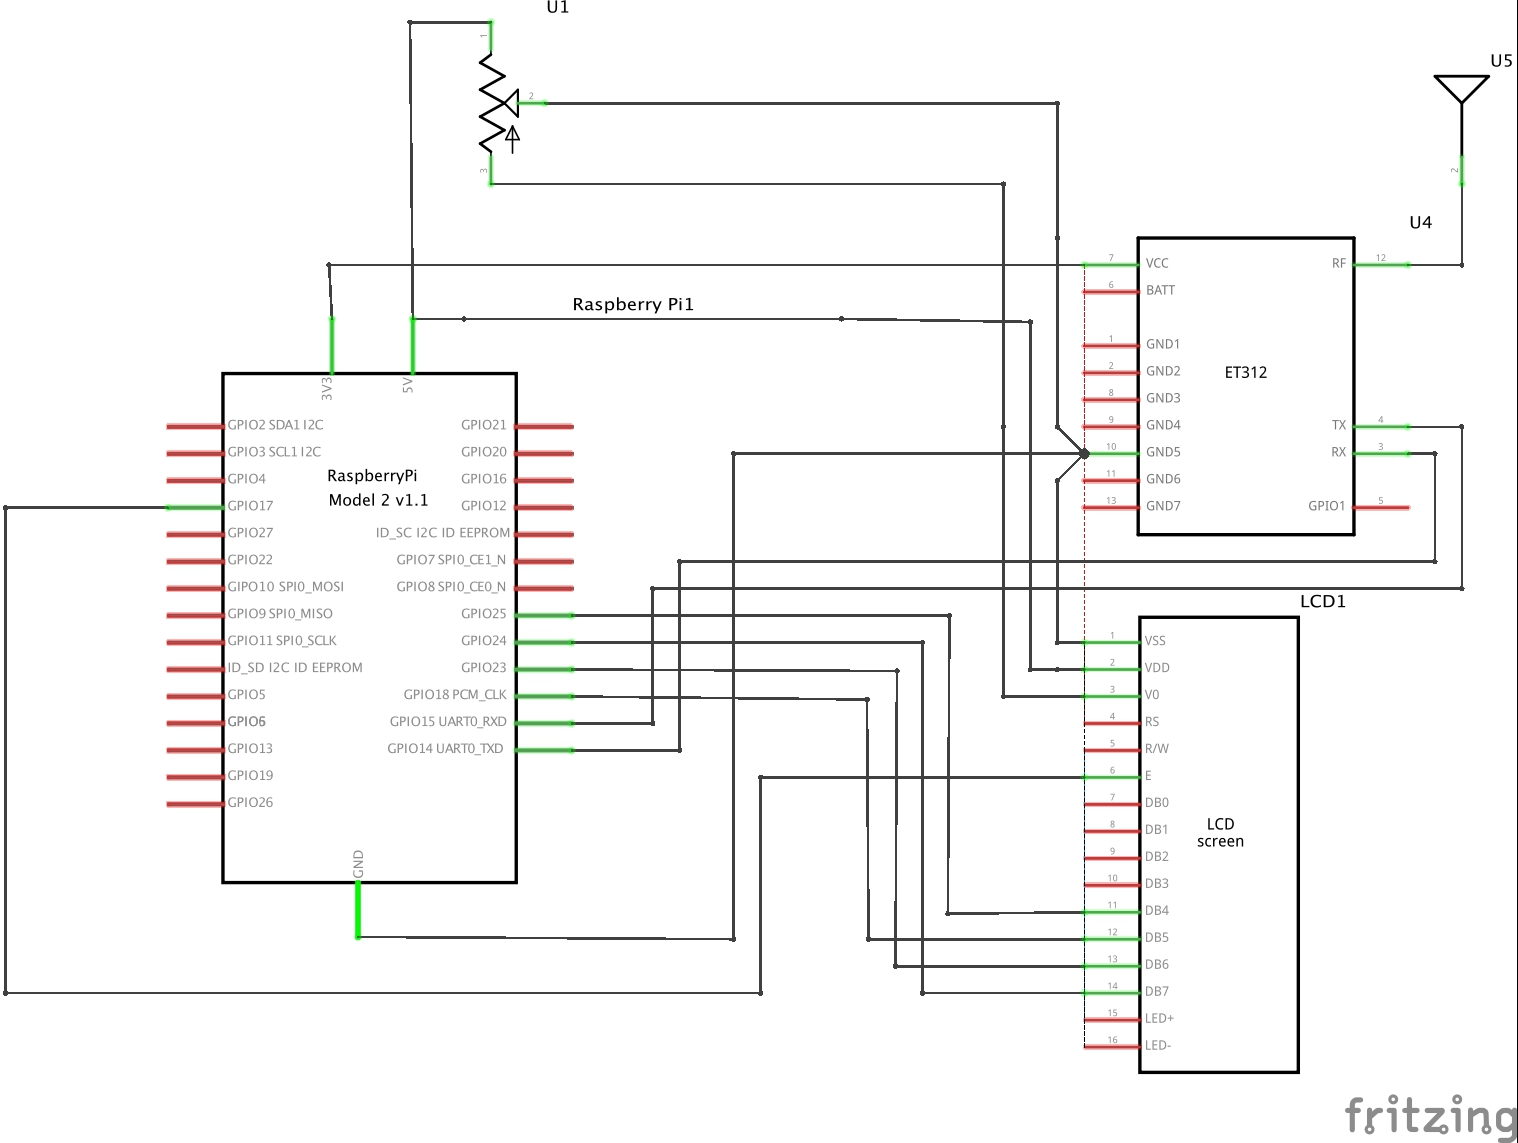
\includegraphics[width=0.9\linewidth]{schemat-podlaczenia_schem.jpg}
			\end{center}
			

		\begin{center}
			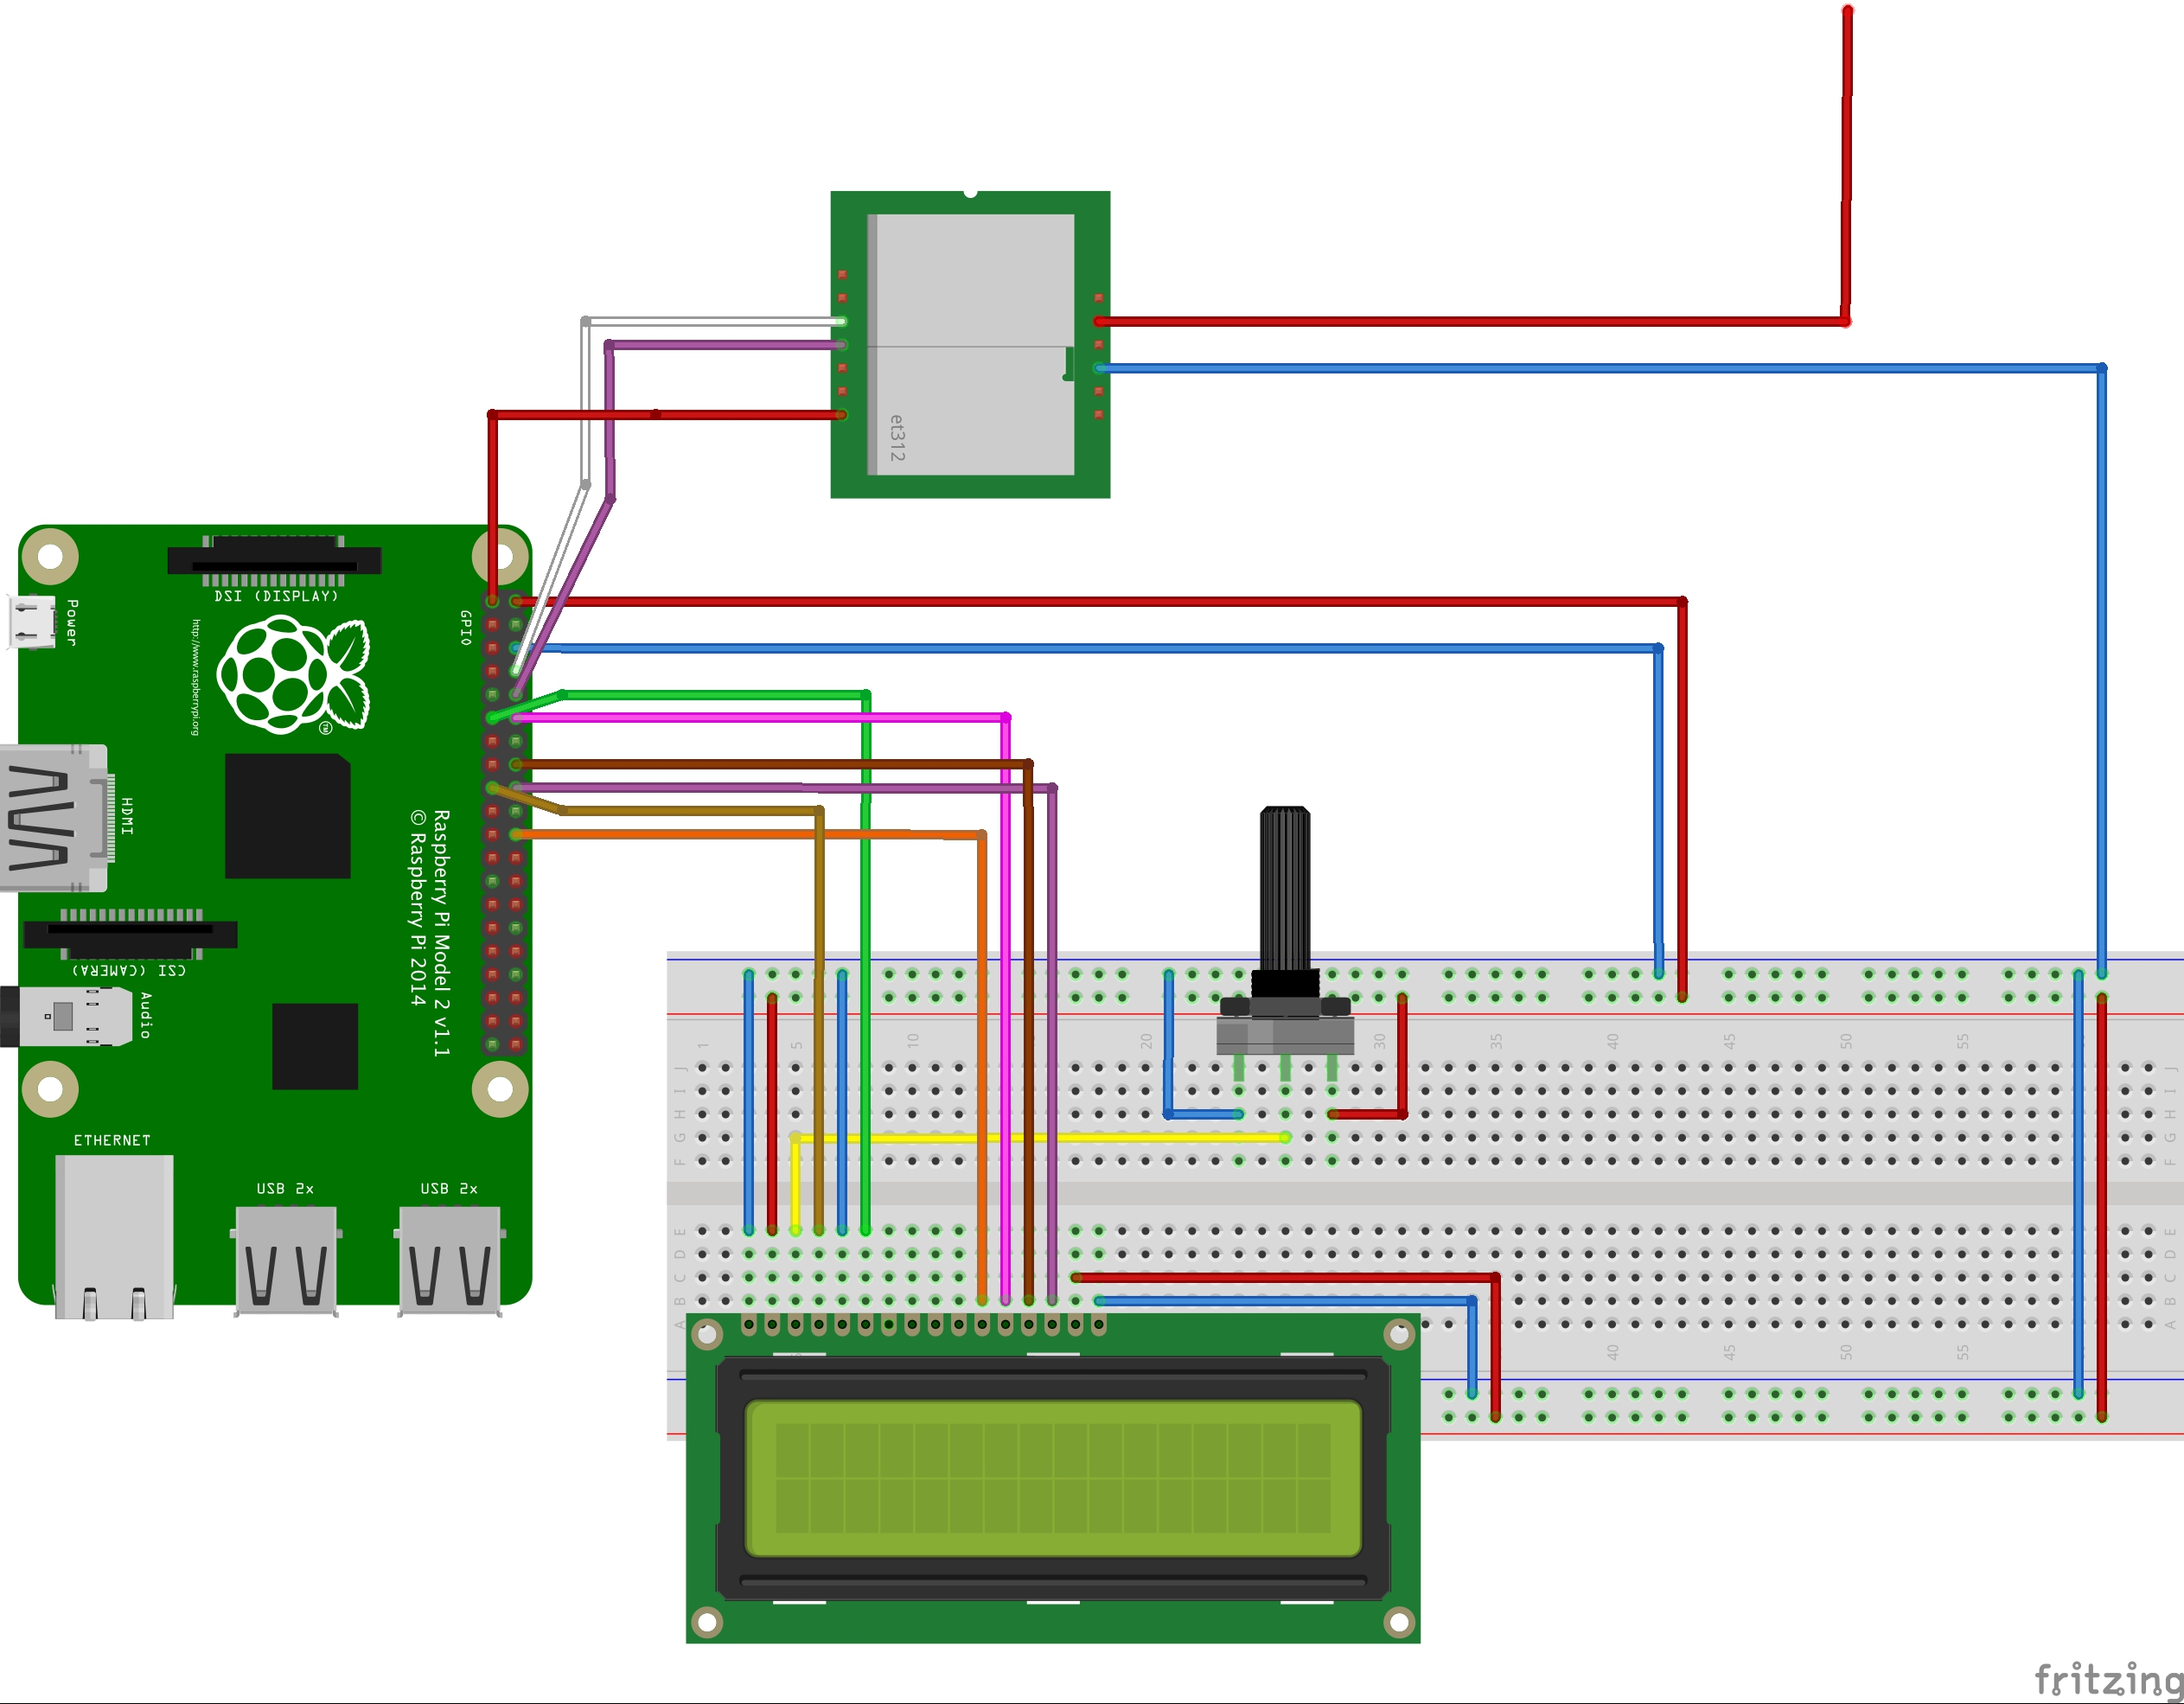
\includegraphics[width=0.9\linewidth]{schemat-podlaczenia_bb.jpg}
		\end{center}
	
\section{Podsumowanie}


\end{document}\documentclass{article}
